%
% File: chap01.tex
% Author: Victor F. Brena-Medina
% Description: Introduction chapter where the biology goes.
%
\let\textcircled=\pgftextcircled
\chapter{Literature Review}
\label{chap:intro}

\initial{S}tress, $\sigma$, is defined as a measure of the force that an object is experiencing per unit of area.\cite{woodford_1993_mechanical} It is well documented that materials can only withstand a certain amount of stress before irreparable deformation occurs \cite{voight_1989_a} \cite{matsuoka_1990_a}, the limit to which is known for almost all industrially utilised materials. \cite{cambridgeuniversityengineeringdepartment_2003_materials} The likelihood of failure for a given component can therefore be inferred from its current stress state.\cite{todinov_2006_equations} In the Nuclear industry, where preventative maintenance is the standard practice and safety case standards demand accurate predictions of the probability of failure for every component \cite{internationalatomicenergyagency_2007_safety}, the ability to infer a material's probability of failure from its residual stress state is valuable. \\

X-Ray diffraction has been used to infer macroscopic residual stress of crystalline materials with high accuracy, precision and low intrusion.\cite{welzel_2005_stress} It follows that this method may be useful in the stress analysis of nuclear materials, and indeed the technique has been used to analyse materials such as steels. \cite{epp_2012_in}\\

 \begin{figure}[h]
 	\centering
 	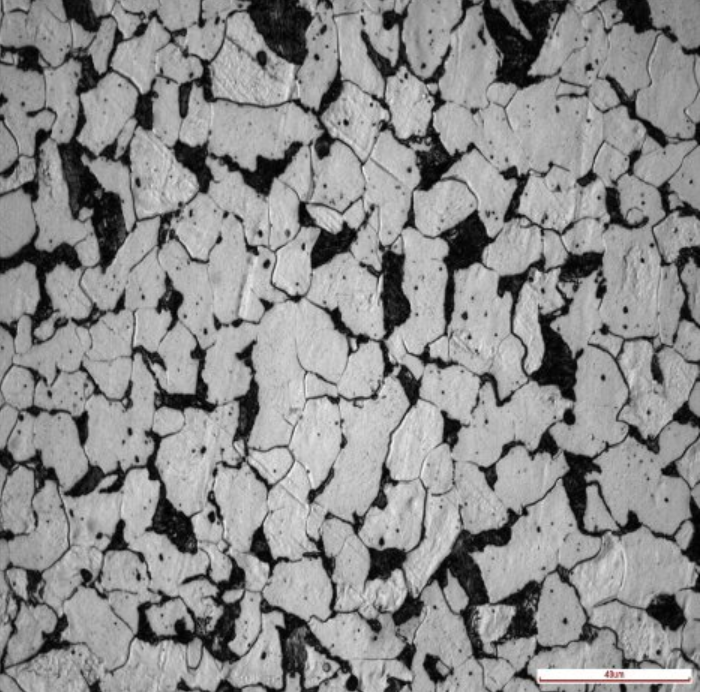
\includegraphics[width=0.6\textwidth]{chapters/chapter01/fig01/microstructure.png}
 	\mycaption[]
 	{Micro structure of Q235 steel. White: Ferrite; Black: Pearlite. \cite{matsuoka_1990_a}}
    \label{fig:RHP02}
 \end{figure}

Numerous materials used in the nuclear industry, such as steels, are alloys \cite{internationalatomicenergyagency_2012_structural} and thus have complex micro structures (figure 2.1). \cite{matsuoka_1990_a} Furthermore, the components can corrode via a combination of several mechanisms due to the harsh and irradiating conditions under which they operate \cite{berg_2009_corrosion}, leading to further non-uniformity in the microstructure.\\ 



Although nuclear materials have been successfully analysed using X-Ray diffraction despite their complex grain structures \cite{shanhua_2015_threedimensional}, the sensitivity of X-Ray diffraction to favourable grain sampling statistics (see section 2.2) resulted in a prerequisite that manual optimisation in the form of peak refinement and anomaly detection was carried out. \cite{scheidegger_2000_correction} This process can be tedious and subjective \cite{he_2018_twodimensional} which may be gating X-Ray diffraction from widespread use in the nuclear industry.\\ 

The sections in this literature review outline the process of stress analysis using X-Ray diffraction (section 2.1) and explain the origin of the technique's sensitivity grain structure (section 2.2). Bayesian statistics are introduced (section 2.3) as a potential solution for difficulties which may arise from unfavourable grain sampling in the X-Ray diffraction of nuclear materials.\\

\section{How Residual Stress Can be Inferred Using X-Ray Diffraction}
\label{sec:sec01}

Bragg scattering is the process which underpins stress analysis using X-Ray diffraction. The scattering angle of a diffracted beam, $\theta$ (figure 2.2), can be used to calculate the distance between lattice planes in a sample. The observed distance can be compared with a known Stress-free lattice spacing, $d_{0}$, to obtain a measure for inter-atomic elongation or compression, i.e a strain measurement for that location. \cite{he_2018_twodimensional}

 \begin{figure}[h]
 	\centering
 	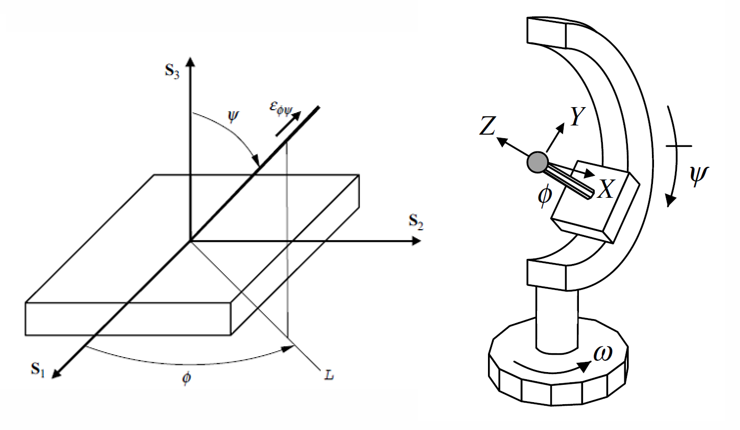
\includegraphics[width=0.6\textwidth]{chapters/chapter01/fig01/diffracion angles.png}
 	\mycaption[]
 	{Strain measurement in a sample's  co-ordinates (left) defined by goniometer (right) angles, $\phi, \omega$ and $\psi$. \cite{he_2018_twodimensional}}
    \label{fig:RHP02}
 \end{figure}

In an unstressed sample, 2$\theta$, is a constant. When a sample is distorted due to stress, 2$\theta$ becomes a function of $\gamma$, $\omega$, $\psi$, and $\phi$. The equation which described the relationship between the strain in a location defined by detector angles and the stress tensor components is as follows: \cite{he_2018_twodimensional}

$$p_{11}\sigma_{11} + p_{12}\sigma_{12}+ p_{22}\sigma_{22}+ p_{13}\sigma_{13}+ p_{23}\sigma_{23}+ p_{33}\sigma_{33} =  \epsilon_{\phi\psi}
$$ \hfill {\bf{Eqn. 1} } \\

Where $\sigma_{11}$ is the stress component in the direction $S_{1}S_{1}$ (figure 2.2) and $p_{ij}$ are stress coefficients, defined in equation 2.\cite{he_2018_twodimensional} 

 \begin{figure}[H]
 	\centering
 	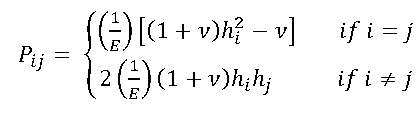
\includegraphics[width=0.4\textwidth]{chapters/chapter01/fig01/pij.png}
%  	\mycaption[]
%  	{Strain measurement in a sample's  co-ordinates (left) defined by goniometer (right) angles, $\phi, \omega$ and $\psi$. }
%     \label{fig:RHP02}
 \end{figure}
\hfill{ \bf{Eqn.2}}\\

Where $\nu$ is the macroscopic Poisson’s ratio, and $h_{i}$ represents a component of the direction of the diffracted beam in the sample co-ordinates, defined in equation 3. \cite{he_2018_twodimensional}

 \begin{figure}[H]
 	\centering
 	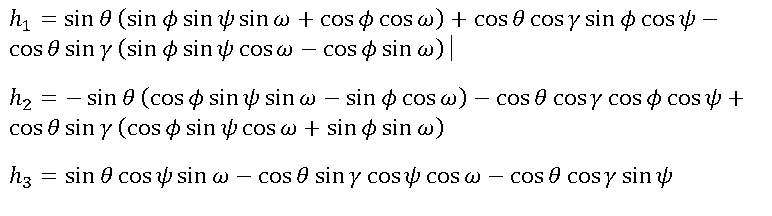
\includegraphics[width=0.8\textwidth]{chapters/chapter01/fig01/h.png}
%  	\mycaption[]
%  	{Strain measurement in a sample's  co-ordinates (left) defined by goniometer (right) angles, $\phi, \omega$ and $\psi$. }
%     \label{fig:RHP02}
 \end{figure}
\hfill{ \bf{Eqn.3}}\\

\section{The Effects of Grain Sampling Statistics}
\label{sec:sec01}

Although the macroscopic stress in a sample is constant \cite{withers_2001_residual}, when measuring stress at several locations in a sample the measurements will vary due to uncertainties in peak position and variation in granular stress (see figure 2.3). 

 \begin{figure}[H]
 	\centering
 	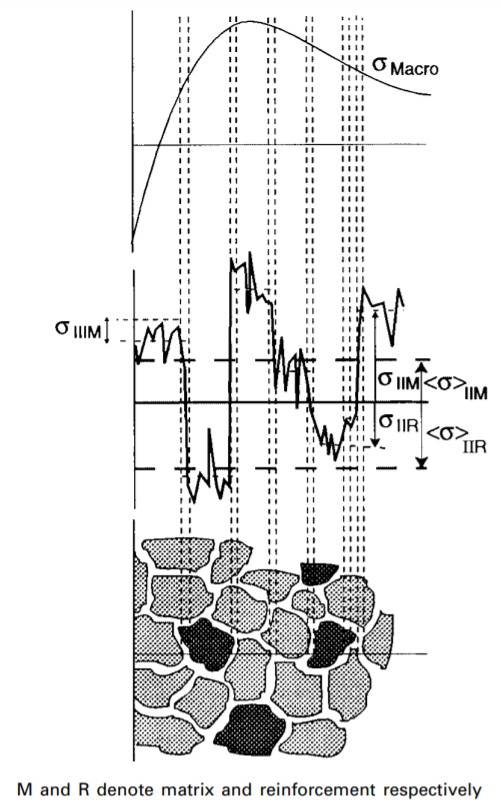
\includegraphics[width=0.6\textwidth]{chapters/chapter01/fig01/grainsamplingstatistics.png}
 	\mycaption[]
 	{An illustration of origins of noise in X-Ray diffraction measurements. If a large grain is sampled, the peak intensity will be high, overshadowing smaller, more representative grains. This can be problematic if the large grain has an abnormally high or low stress \cite{withers_2001_residual}}
    \label{fig:RHP02}
 \end{figure}

The uncertainty associated with peak position can be easily resolves using peak width analysis \cite{luo_2017_uncertainty} and is therefore often known, however the uncertainty arising from grain sampling is unknown. Furthermore, only grains in an appropriate orientation will allow for Bragg diffraction to be observed \cite{bramble_2014_grain}, due to the requirement for constructive interference with the X-Ray. Therefore, poor grain sampling can also result in 'spotty' and sparse diffraction measurements, as illustrated in figure 2.4. 

 \begin{figure}[H]
 	\centering
 	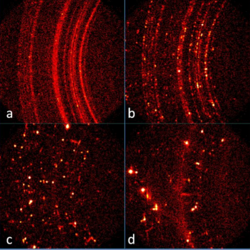
\includegraphics[width=0.6\textwidth]{chapters/chapter01/fig01/spotty.png}
 	\mycaption[]
 	{a) Debye Ring, b-c) Increasingly sparse data caused by poor grain sampling; it is no longer possible to see the Debye ring and measure its radius to obtain 2$\theta$ . \cite{bramble_2014_grain} }
    \label{fig:RHP02}
 \end{figure}



\section{Bayesian Statistics Applied to Stress Analysis}
\label{sec:sec01}


